\section{Kadek Diva Krishna Murti}
\subsection{Soal 1}
Buatlah  fungsi  (file  terpisah/library  dengan  nama  NPMcsv.py)  untuk  membuka file csv dengan lib csv mode list.

\lstinputlisting[caption = Fungsi untuk membuka file CSV dengan lib CSV mode list., firstline=10, lastline=15]{src/4/1174006/Praktek/1174006csv.py}

\subsection{Soal 2}
Buatlah  fungsi  (file  terpisah/library  dengan  nama  NPMcsv.py)  untuk  membuka file csv dengan lib csv mode dictionary.

\lstinputlisting[caption =  Fungsi untuk membuka file CSV dengan lib CSV mode dictionary., firstline=17, lastline=22]{src/4/1174006/Praktek/1174006csv.py}

\subsection{Soal 3}
Buatlah fungsi (file terpisah/library dengan nama NPMpandas.py) untuk membuka file csv dengan lib pandas mode list.

\lstinputlisting[caption =  Fungsi untuk membuka file CSV dengan lib Pandas mode list., firstline=10, lastline=13]{src/4/1174006/Praktek/1174006pandas.py}

\subsection{Soal 4}
Buatlah fungsi (file terpisah/library dengan nama NPMpandas.py) untuk membuka file csv dengan lib pandas mode dictionary.

\lstinputlisting[caption =  Fungsi untuk membuka file CSV dengan lib Pandas mode dictionary., firstline=10, lastline=13]{src/4/1174006/Praktek/1174006pandas.py}

\subsection{Soal 5}
Buat fungsi baru di NPMpandas.py untuk mengubah format tanggal menjadi standar dataframe.

\lstinputlisting[caption =  Fungsi untuk mengubah format tanggal menjadi standar dataframe., firstline=15, lastline=19]{src/4/1174006/Praktek/1174006pandas.py}

\subsection{Soal 6}
Buat fungsi baru di NPMpandas.py untuk mengubah index kolom.

\lstinputlisting[caption =  Fungsi untuk mengubah index kolom., firstline=21, lastline=24]{src/4/1174006/Praktek/1174006pandas.py}

\subsection{Soal 7}
Buat fungsi baru di NPMpandas.py untuk mengubah atribut atau nama kolom.

\lstinputlisting[caption =  Fungsi untuk mengubah atribut atau nama kolom., firstline=26, lastline=30]{src/4/1174006/Praktek/1174006pandas.py}

\subsection{Soal 8}
Buat program main.py yang menggunakan library NPMcsv.py yang membuat dan membaca file csv.

\lstinputlisting[caption =  Membuat dan mebaca file CSV menggunakan library 1174006pandas., firstline=8, lastline=13]{src/4/1174006/Praktek/main.py}

\subsection{Soal 9}
Buat program main2.py yang menggunakan library NPMpandas.py yang membuat dan membaca file csv.

\lstinputlisting[caption = Membuat dan mmebaca file CSV menggunakan library 1174006pandas., firstline=8, lastline=13]{src/4/1174006/Praktek/main2.py}

\subsection{Kode Program Praktek}
\begin{figure}[H]
	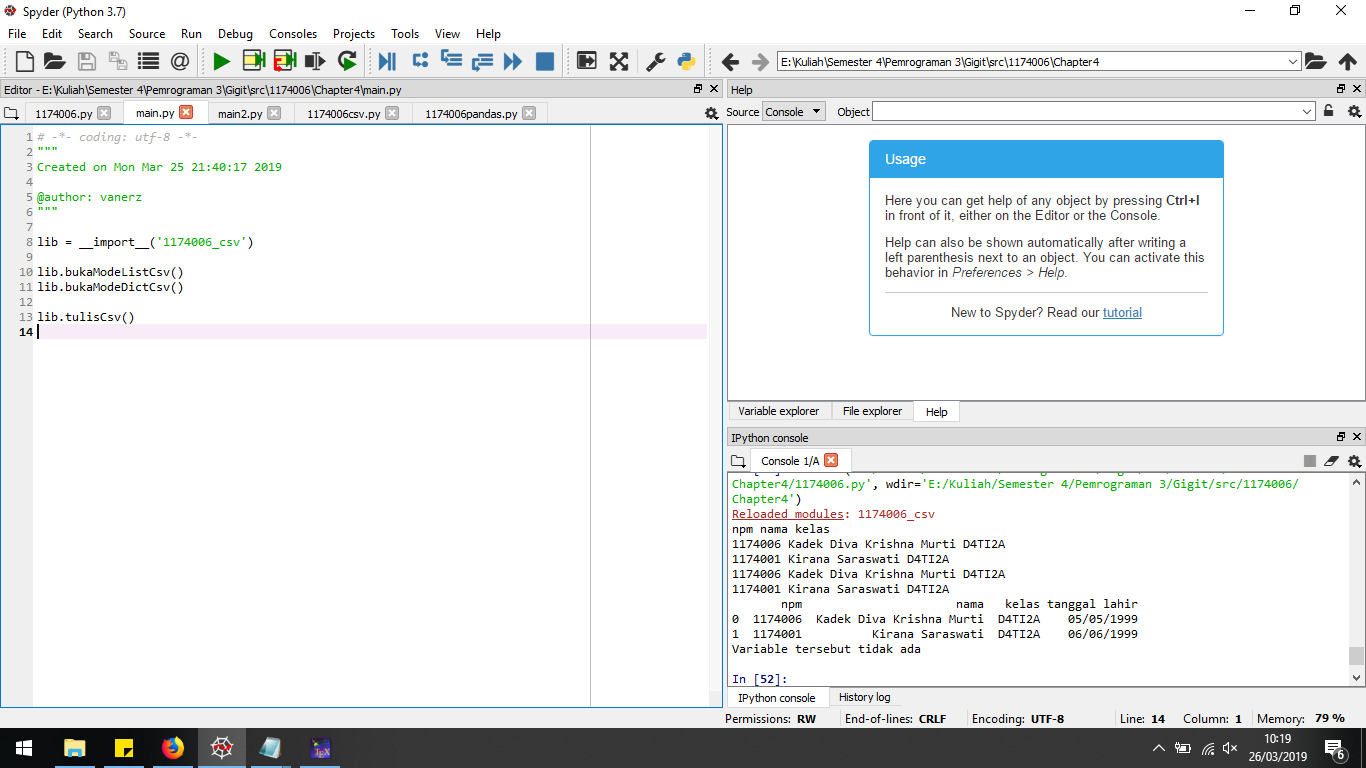
\includegraphics[width=9cm]{figures/4/1174006/Praktek/k1.png}
	\centering
\end{figure}
\begin{figure}[H]
	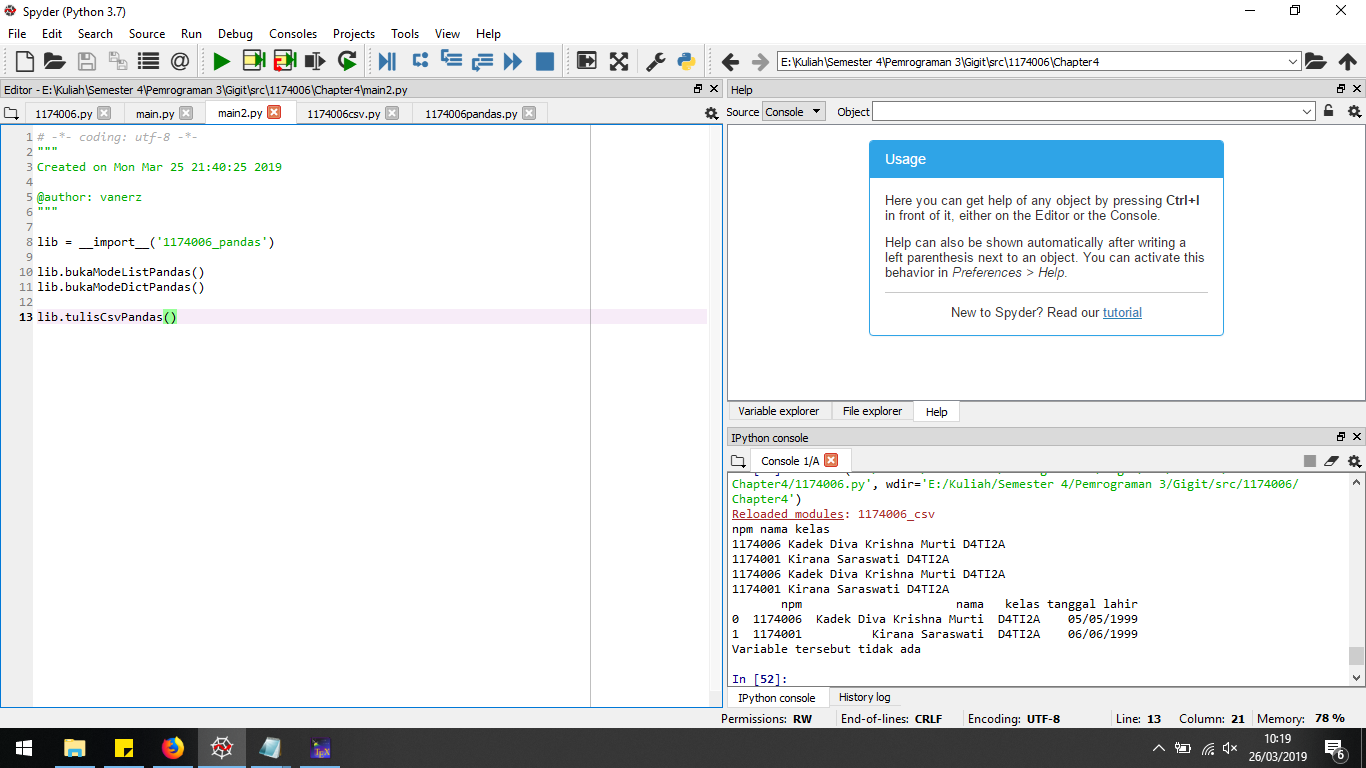
\includegraphics[width=10cm]{figures/4/1174006/Praktek/k2.png}
	\centering
\end{figure}
\begin{figure}[H]
	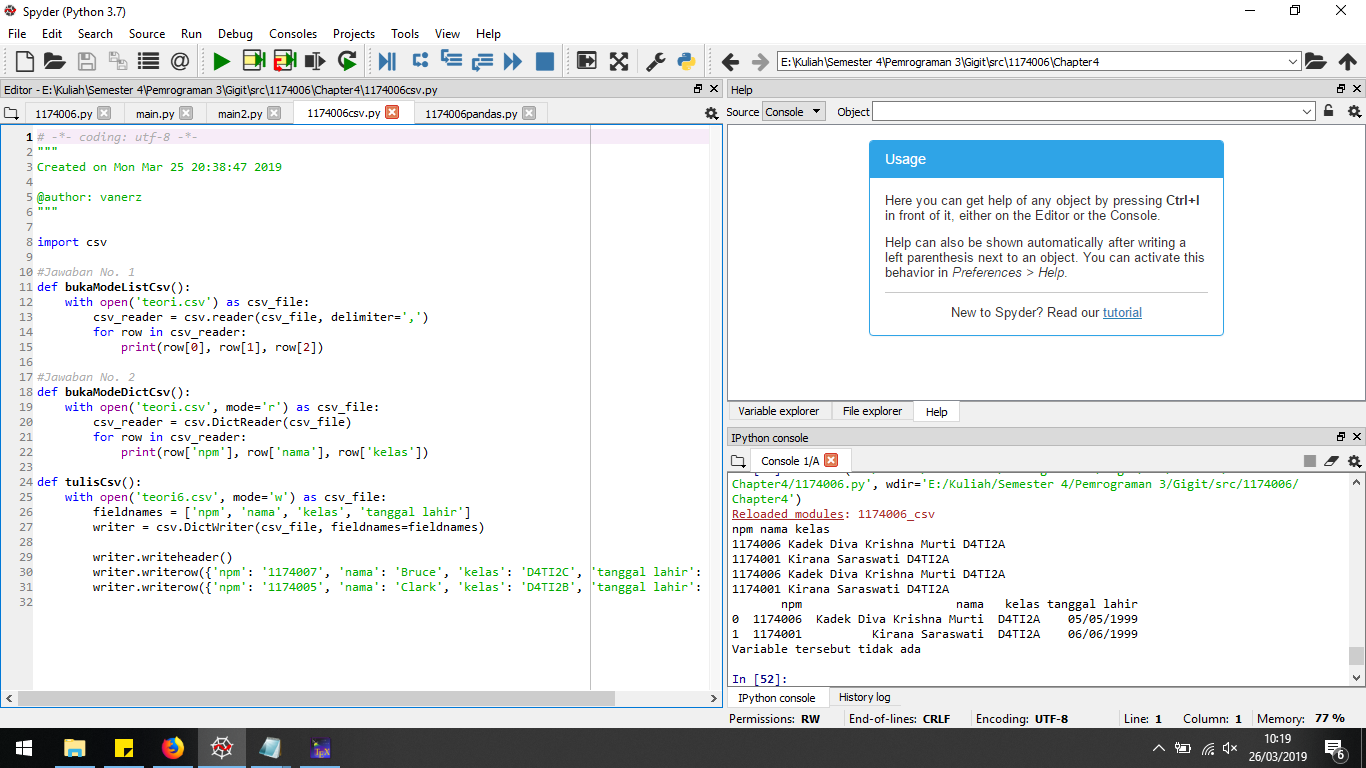
\includegraphics[width=10cm]{figures/4/1174006/Praktek/k3.png}
	\centering
\end{figure}
\begin{figure}[H]
	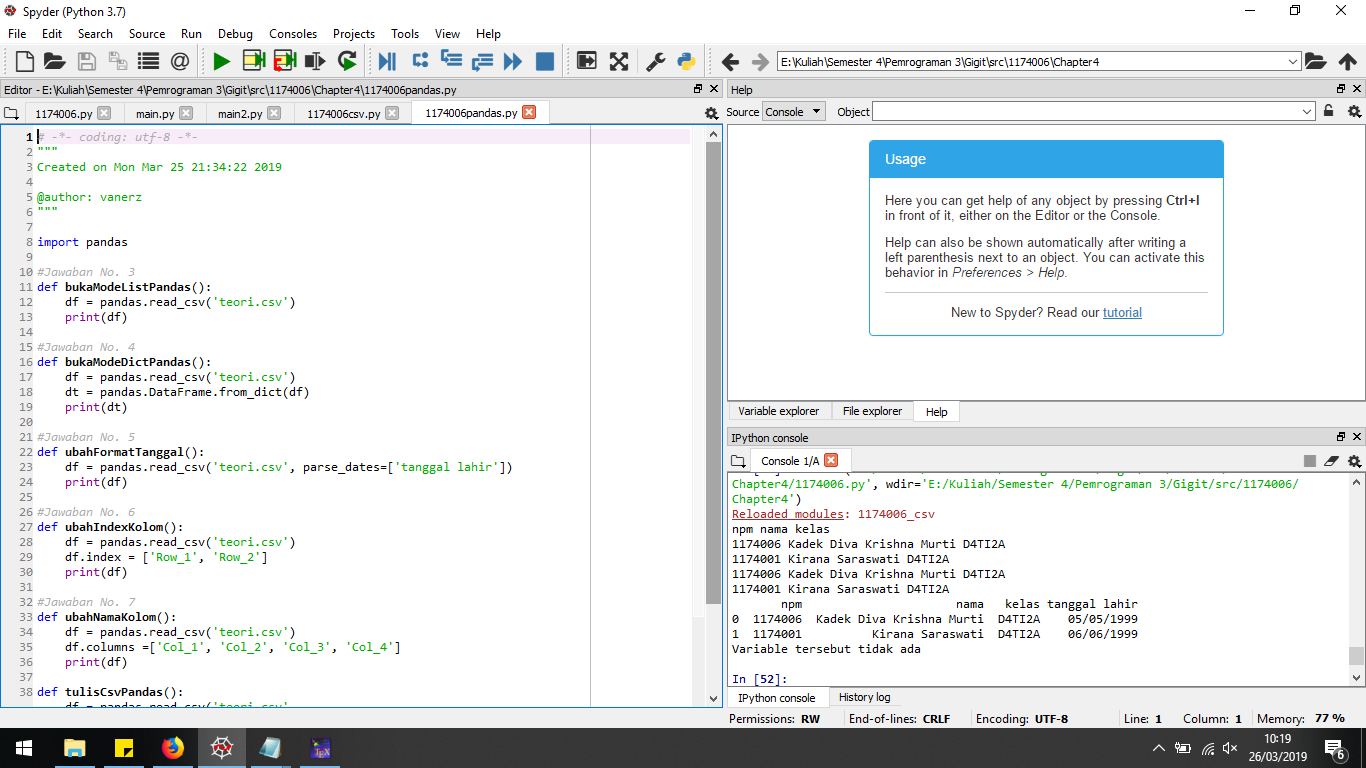
\includegraphics[width=9cm]{figures/4/1174006/Praktek/k4.png}
	\centering
\end{figure}
\begin{figure}[H]
	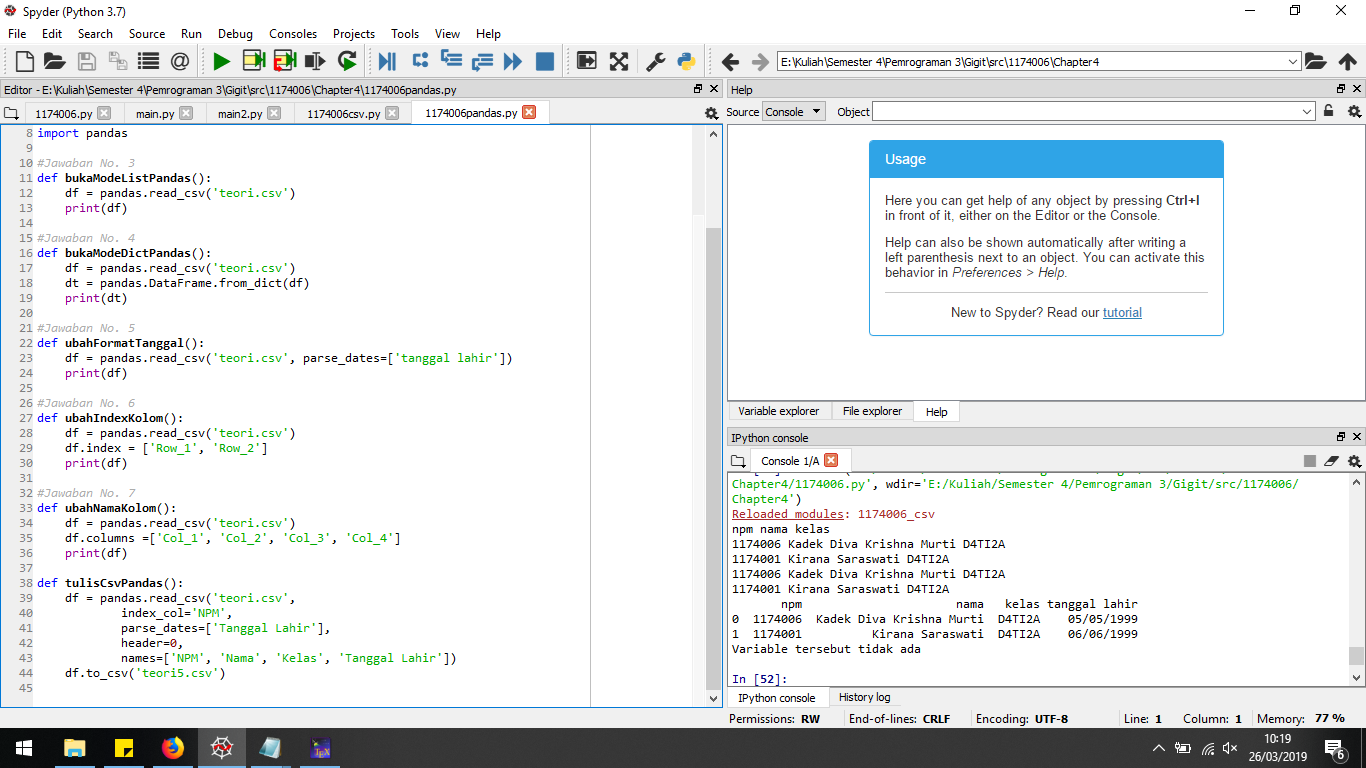
\includegraphics[width=10cm]{figures/4/1174006/Praktek/k5.png}
	\centering
\end{figure}

\subsection{Cek Plagiat Praktek}
\begin{figure}[H]
	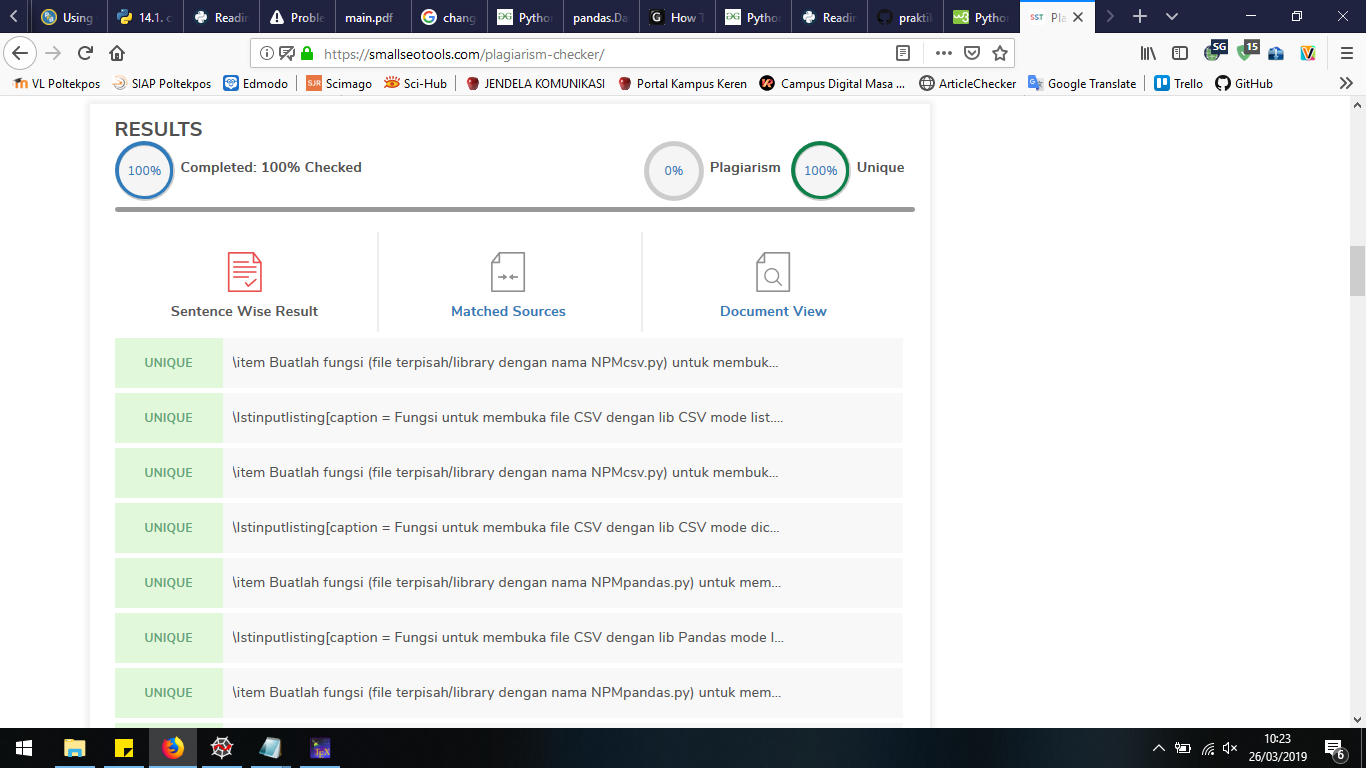
\includegraphics[width=10cm]{figures/4/1174006/Praktek/plagiatketrampilan.png}
	\centering
\end{figure}

\subsection{Soal 1}
Tuliskan  peringatan  error  yang  didapat  dari  mengerjakan  praktek  keempat  ini, dan  jelaskan  cara  penanganan  error  tersebut.   dan  Buatlah  satu  fungsi  yang menggunakan gunakan try except untuk menanggulangi error tersebut.

Peringatan error di praktek keempat ini, yaitu:
\begin{itemize}
	\item Syntax Errors
	Syntax Errors adalah suatu keadaan saat kode python mengalami kesalahan penulisan. Solusinya adalah memperbaiki penulisan kode yang salah.
	
	\item Name Error
	NameError adalah exception yang terjadi saat kode melakukan eksekusi terhadap local name atau global name yang tidak terdefinisi. Solusinya adalah memastikan variabel atau function yang dipanggil ada atau tidak salah ketik.
	
	\item Type Error
	TypeError adalah exception yang akan terjadi apabila pada saat dilakukannya eksekusi terhadap suatu operasi atau fungsi dengan type object yang tidak sesuai. Solusi dari error ini adalah mengkoversi varibelnya sesuai dengan tipe data yang akan digunakan.
\end{itemize}

Fungsi yang menggunakan try except
\lstinputlisting[caption= Fungsi yang menggunakan try except .,firstline=55, lastline=67]{src/4/1174006/Teori/1174006.py}

\subsection{Kode Program Penanganan Error}
\begin{figure}[H]
	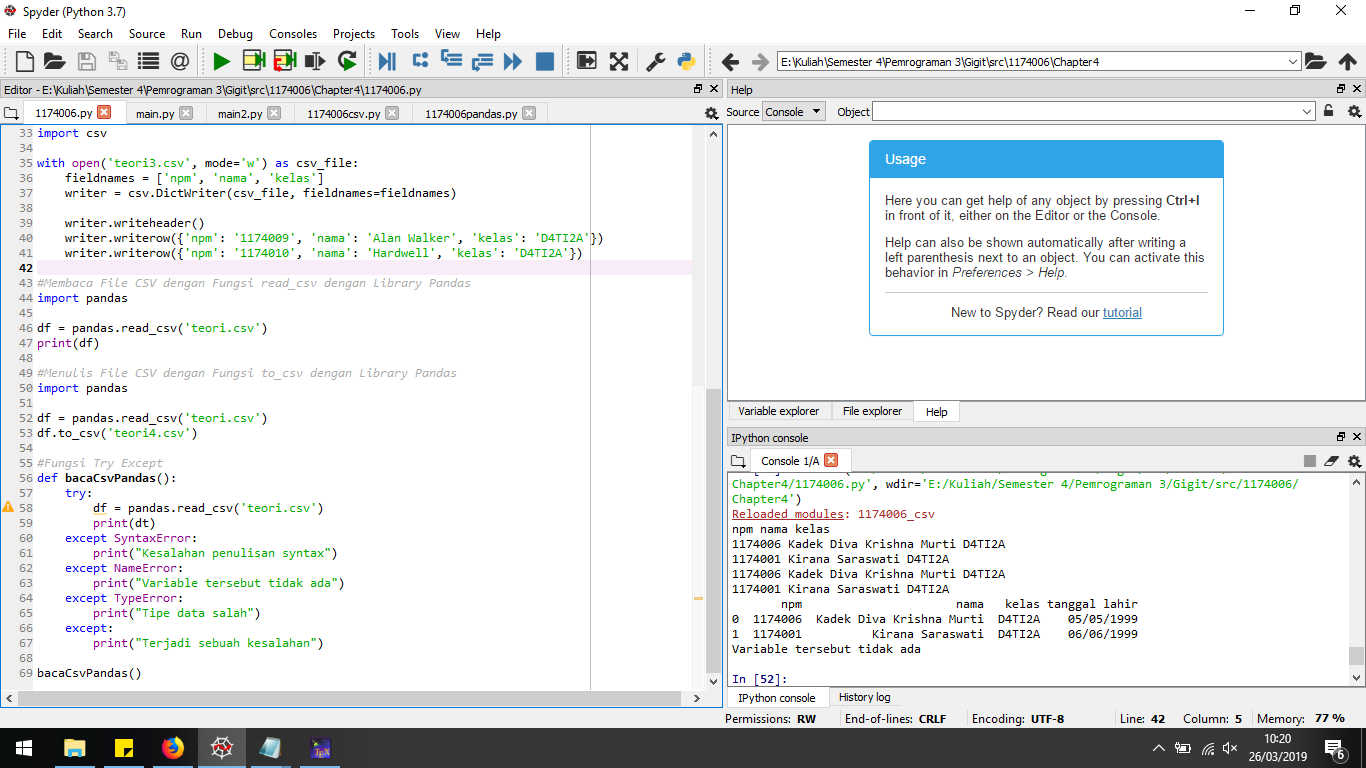
\includegraphics[width=10cm]{figures/4/1174006/Praktek/p1.png}
	\centering
\end{figure}

\subsection{Plagiat Penanganan Error}
\begin{figure}[H]
	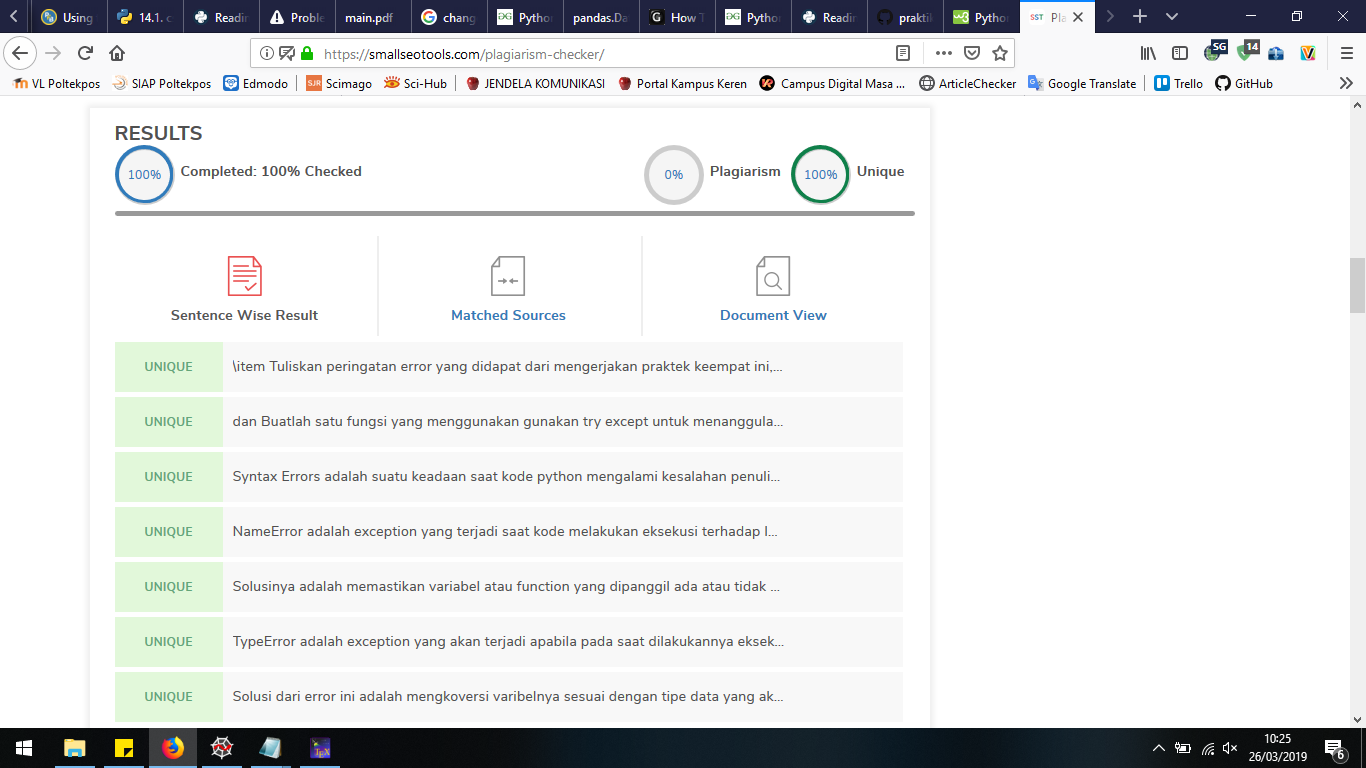
\includegraphics[width=10cm]{figures/4/1174006/Praktek/plagiatpenanganan.png}
	\centering
\end{figure}

%%%%%%%%%%%%%%%%%%%%%%%%%%%%%%%%%%%%%%%%%%%%%%%%%%%%%%%%%%%%%%%%%%%%

\section{Damara Benedikta}
\subsection{Soal 1}
Berikut adalah pemanggilan file csv dengan library csv yang menggunakan list
\lstinputlisting[firstline=10, lastline=20]{src/4/1174012/praktek/c_1174012_csv.py}

\subsection{Soal 2}
Berikut adalah pemanggilan file csv dengan library csv yang menggunakan dictionary
\lstinputlisting[firstline=22, lastline=31]{src/4/1174012/praktek/c_1174012_csv.py}

\subsection{Soal 3}
Berikut adalah pemanggilan file csv dengan library pandas yang menggunakan list
\lstinputlisting[firstline=9, lastline=11]{src/4/1174012/praktek/p_1174012_pandas.py}

\subsection{Soal 4}
Berikut adalah pemanggilan file csv dengan library pandas yang menggunakan dictionary
\lstinputlisting[firstline=13, lastline=16]{src/4/1174012/praktek/p_1174012_pandas.py}

\subsection{Soal 5}
Berikut penggunaan untuk merubah standar penulisan tanggal, yang mengikuti standar penulisan dari pandas.
\lstinputlisting[firstline=18, lastline=20]{src/4/1174012/praktek/p_1174012_pandas.py}

\subsection{Soal 6}
Berikut merupakan pergantian index kolom
\lstinputlisting[firstline=22, lastline=24]{src/4/1174012/praktek/p_1174012_pandas.py}

\subsection{Soal 7}
berikut merupakan penggunaan untuk merename atribut yang digunakan, atau merubah nama header 0
\lstinputlisting[firstline=26, lastline=30]{src/4/1174012/praktek/p_1174012_pandas.py}

\subsection{Soal 8}
\lstinputlisting[firstline=8, lastline=10]{src/4/1174012/praktek/main_damara.py}

\subsection{Soal 9}
\lstinputlisting[firstline=11, lastline=14]{src/4/1174012/praktek/main_damara.py}

\subsection{Penanganan Error}
Tidak ada error
%%%%%%%%%%%%%%%%%%%%%%%%%%%%%%%%%%%%%%%%%%%%%%%%%%%%
\section{Felix Setiawan Lase}
\subsection{Soal 1}
Buatlah  fungsi  (file  terpisah/library  dengan  nama  NPMcsv.py)  untuk  membuka file csv dengan lib csv mode list.

\lstinputlisting[caption = Fungsi untuk membuka file CSV dengan lib CSV mode list., firstline=10, lastline=15]{src/4/1174026/Praktek/1174026_csv.py}

\subsection{Soal 2}
Buatlah  fungsi  (file  terpisah/library  dengan  nama  NPMcsv.py)  untuk  membuka file csv dengan lib csv mode dictionary.

\lstinputlisting[caption =  Fungsi untuk membuka file CSV dengan lib CSV mode dictionary., firstline=17, lastline=22]{src/4/1174026/Praktek/1174026_csv.py}

\subsection{Soal 3}
Buatlah fungsi (file terpisah/library dengan nama NPMpandas.py) untuk membuka file csv dengan lib pandas mode list.

\lstinputlisting[caption =  Fungsi untuk membuka file CSV dengan lib Pandas mode list., firstline=10, lastline=13]{src/4/1174026/Praktek/1174026_pandas.py}

\subsection{Soal 4}
Buatlah fungsi (file terpisah/library dengan nama NPMpandas.py) untuk membuka file csv dengan lib pandas mode dictionary.

\lstinputlisting[caption =  Fungsi untuk membuka file CSV dengan lib Pandas mode dictionary., firstline=10, lastline=13]{src/4/1174026/Praktek/1174026_pandas.py}

\subsection{Soal 5}
Buat fungsi baru di NPMpandas.py untuk mengubah format tanggal menjadi standar dataframe.

\lstinputlisting[caption =  Fungsi untuk mengubah format tanggal menjadi standar dataframe., firstline=15, lastline=19]{src/4/1174026/Praktek/1174026_pandas.py}

\subsection{Soal 6}
Buat fungsi baru di NPMpandas.py untuk mengubah index kolom.

\lstinputlisting[caption =  Fungsi untuk mengubah index kolom., firstline=21, lastline=24]{src/4/1174026/Praktek/1174026_pandas.py}

\subsection{Soal 7}
Buat fungsi baru di NPMpandas.py untuk mengubah atribut atau nama kolom.

\lstinputlisting[caption =  Fungsi untuk mengubah atribut atau nama kolom., firstline=26, lastline=30]{src/4/1174026/Praktek/1174026_pandas.py}

\subsection{Soal 8}
Buat program main.py yang menggunakan library NPMcsv.py yang membuat dan membaca file csv.

\lstinputlisting[caption =  Membuat dan mebaca file CSV menggunakan library 1174006pandas., firstline=8, lastline=13]{src/4/1174026/Praktek/main.py}

\subsection{Soal 9}
Buat program main2.py yang menggunakan library NPMpandas.py yang membuat dan membaca file csv.

\lstinputlisting[caption = Membuat dan mmebaca file CSV menggunakan library 1174006pandas., firstline=8, lastline=13]{src/4/1174026/Praktek/main2.py}

\subsection{Kode Program Praktek}
\begin{figure}[H]
	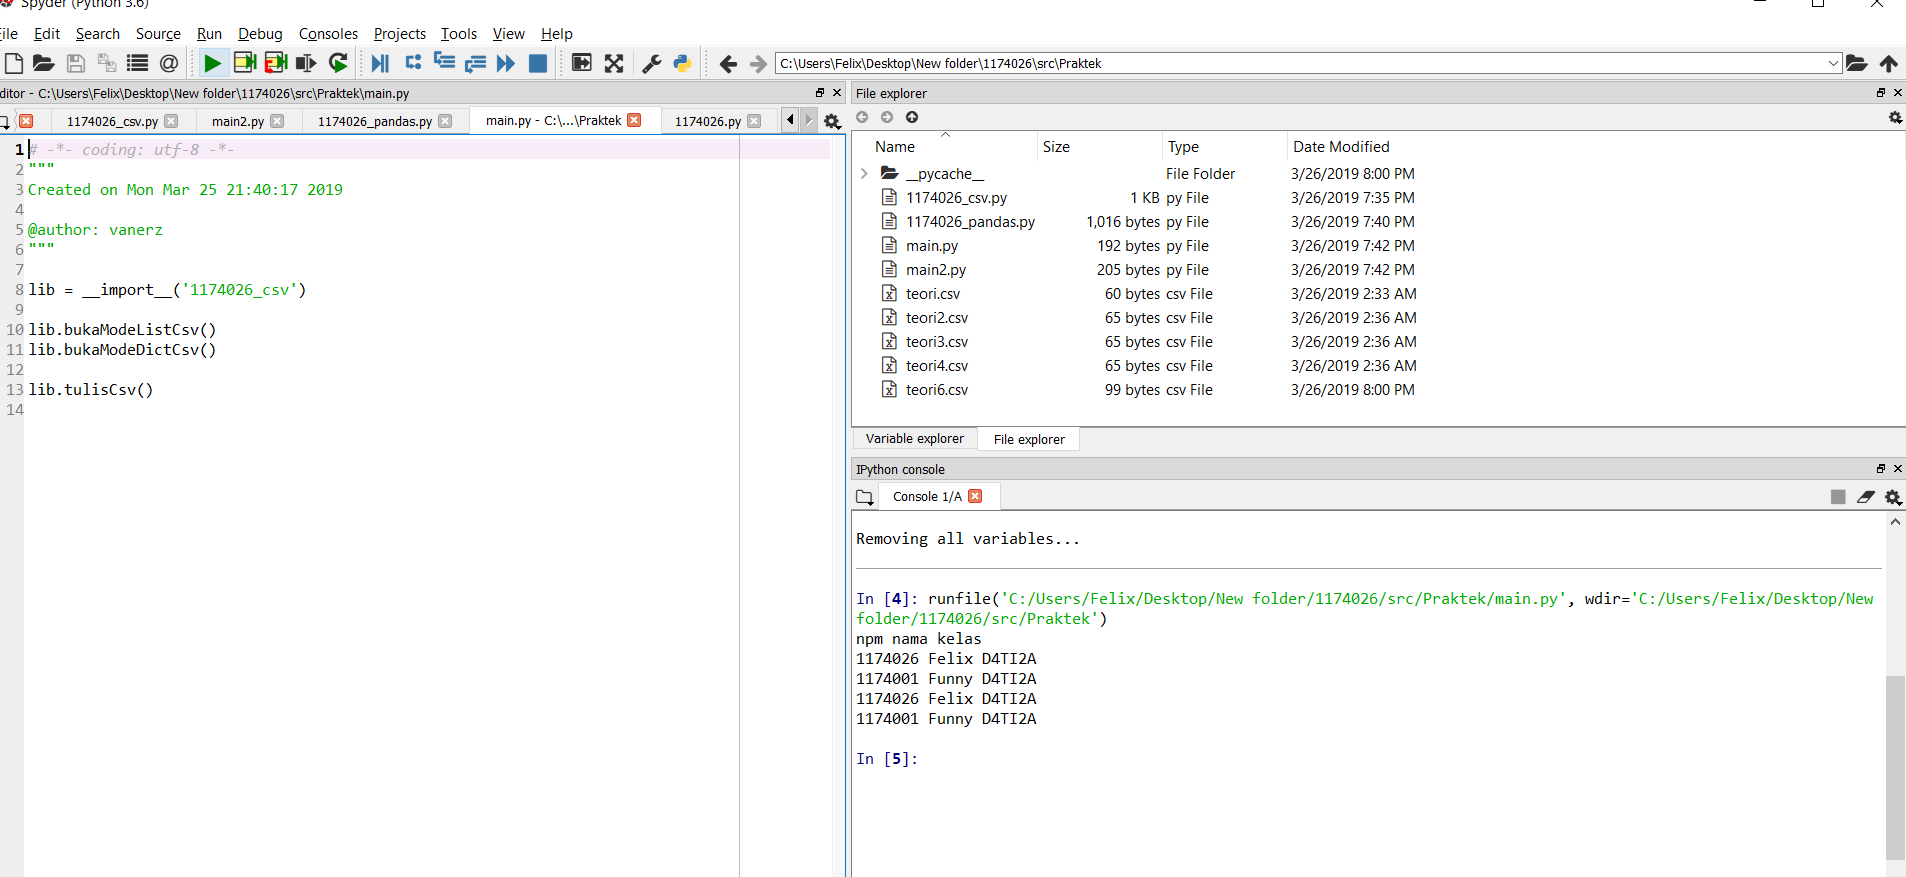
\includegraphics[width=9cm]{figures/4/1174026/Praktek/k1.png}
	\centering
\end{figure}
\begin{figure}[H]
	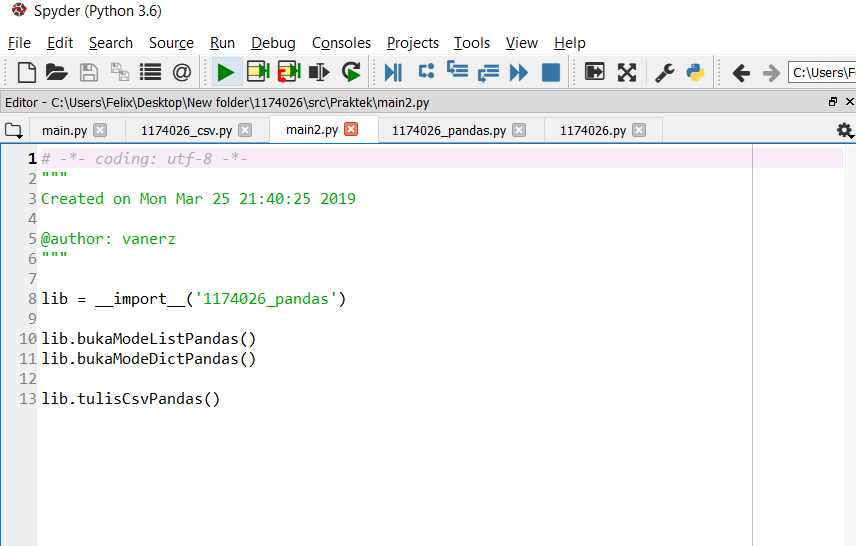
\includegraphics[width=10cm]{figures/4/1174026/Praktek/k2.png}
	\centering
\end{figure}
\begin{figure}[H]
	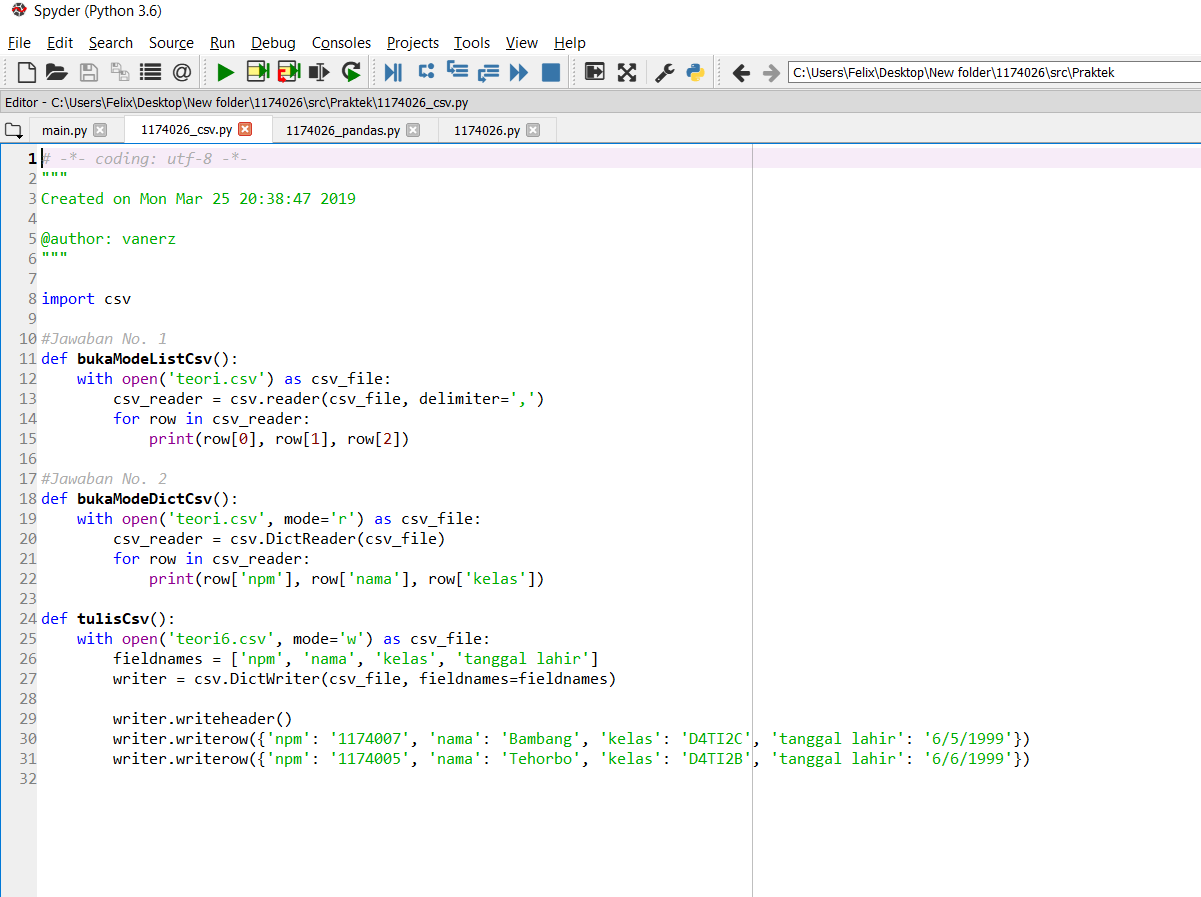
\includegraphics[width=10cm]{figures/4/1174026/Praktek/k3.png}
	\centering
\end{figure}
\begin{figure}[H]
	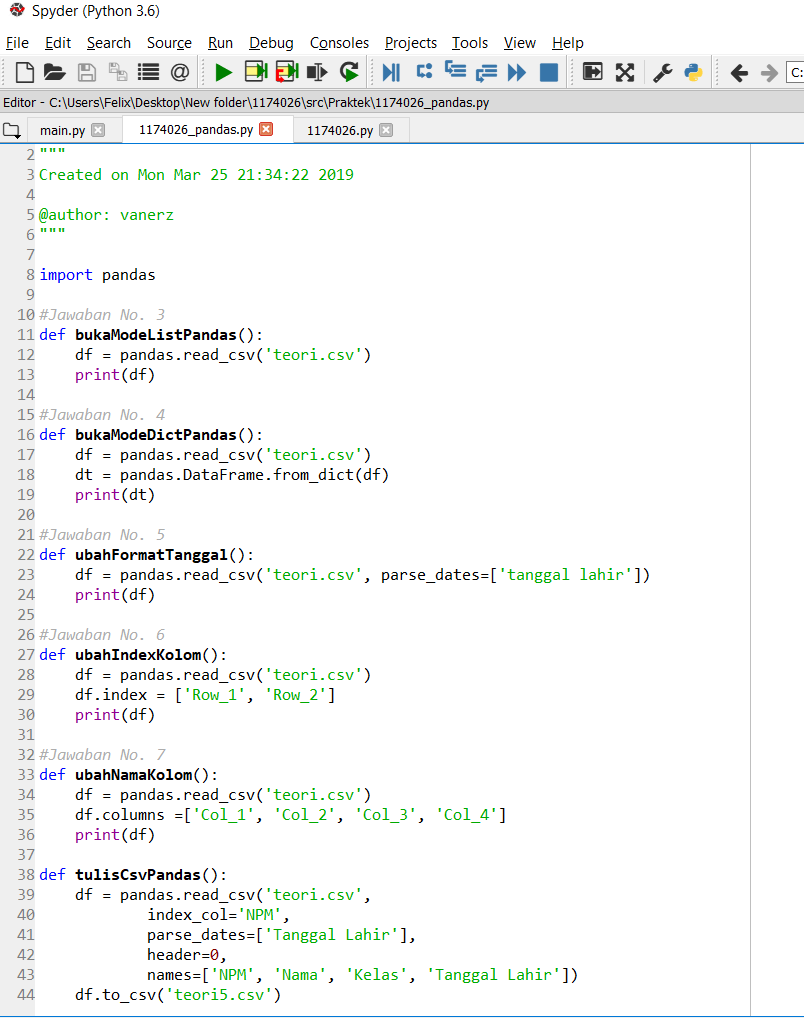
\includegraphics[width=9cm]{figures/4/1174026/Praktek/k4.png}
	\centering
\end{figure}
\begin{figure}[H]
	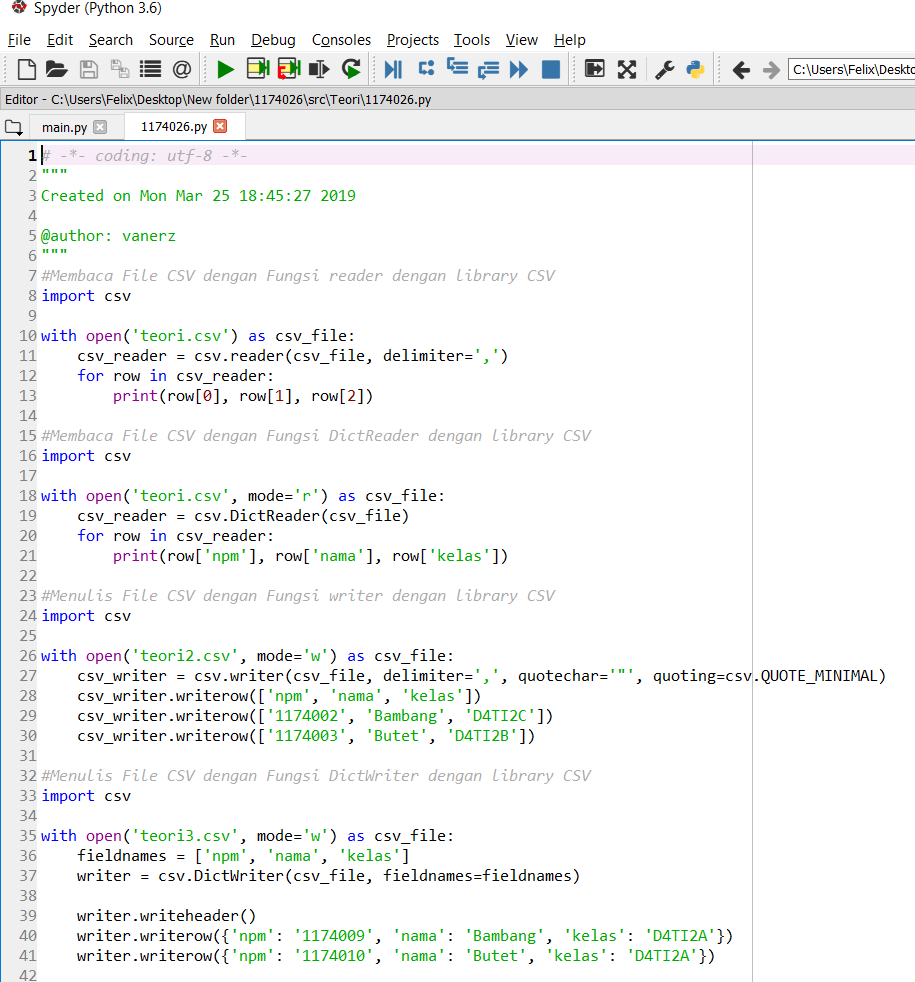
\includegraphics[width=10cm]{figures/4/1174026/Praktek/k5.png}
	\centering
\end{figure}

\subsection{Cek Plagiat Praktek}
\begin{figure}[H]
	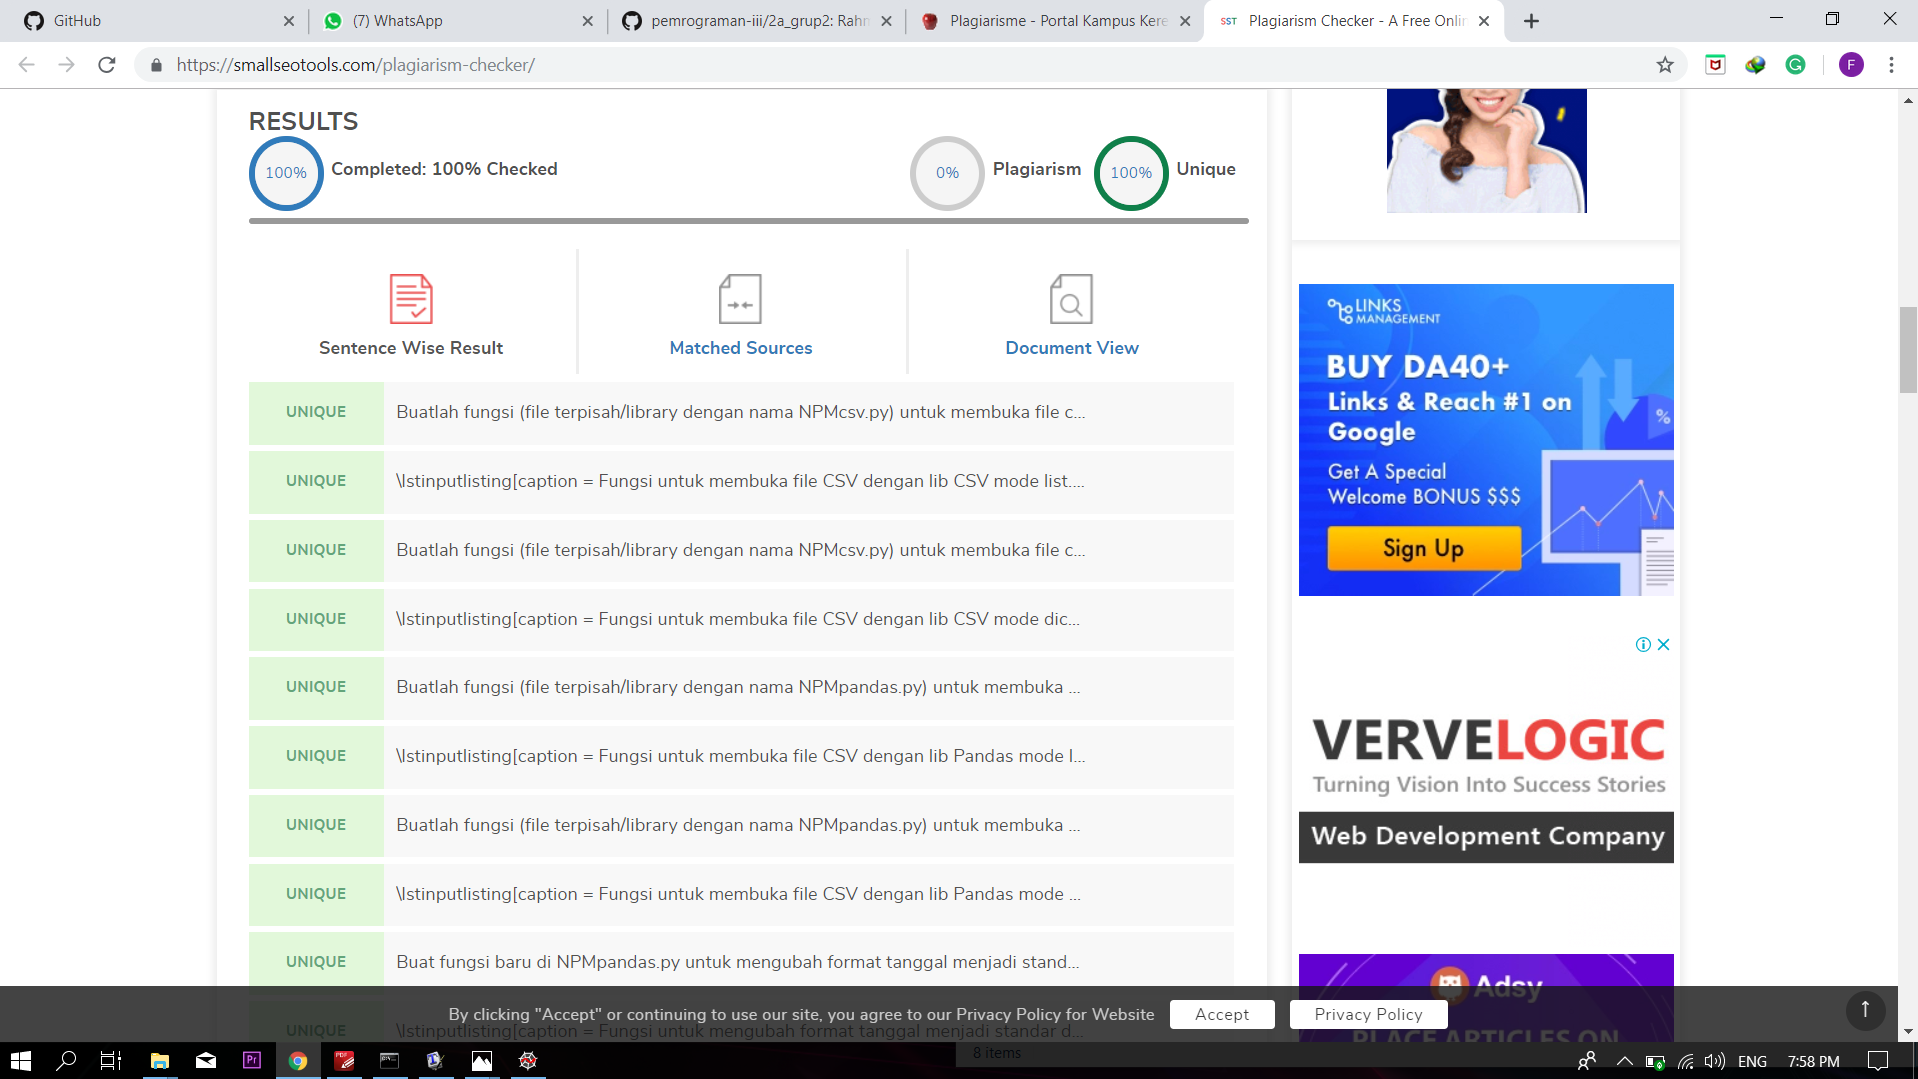
\includegraphics[width=10cm]{figures/4/1174026/Praktek/plagiatketerampilan.png}
	\centering
\end{figure}

\subsection{Soal 1}
Tuliskan  peringatan  error  yang  didapat  dari  mengerjakan  praktek  keempat  ini, dan  jelaskan  cara  penanganan  error  tersebut.   dan  Buatlah  satu  fungsi  yang menggunakan gunakan try except untuk menanggulangi error tersebut.

Peringatan error di praktek keempat ini, yaitu:
\begin{itemize}
	\item Syntax Errors
	Kesalahan Sintaksis adalah suatu kondisi ketika kode python mengalami kesalahan penulisan. Solusinya adalah memperbaiki penulisan kode yang salah.
	
	\item Name Error
	NameError adalah pengecualian yang terjadi ketika kode mengeksekusi nama lokal atau nama global yang tidak ditentukan. Solusinya adalah memastikan variabel atau fungsi yang dipanggil ada atau tidak salah ketik.
	
	\item Type Error
	TypeError adalah pengecualian yang akan terjadi jika eksekusi operasi atau fungsi dengan tipe objek tidak sesuai ketika dieksekusi. Solusi untuk kesalahan ini adalah mengubah variabel sesuai dengan tipe data yang akan digunakan.
\end{itemize}

Fungsi yang menggunakan try except
\lstinputlisting[caption= Fungsi yang menggunakan try except .,firstline=55, lastline=67]{src/4/1174006/Teori/1174026.py}

\subsection{Kode Program Penanganan Error}
\begin{figure}[H]
	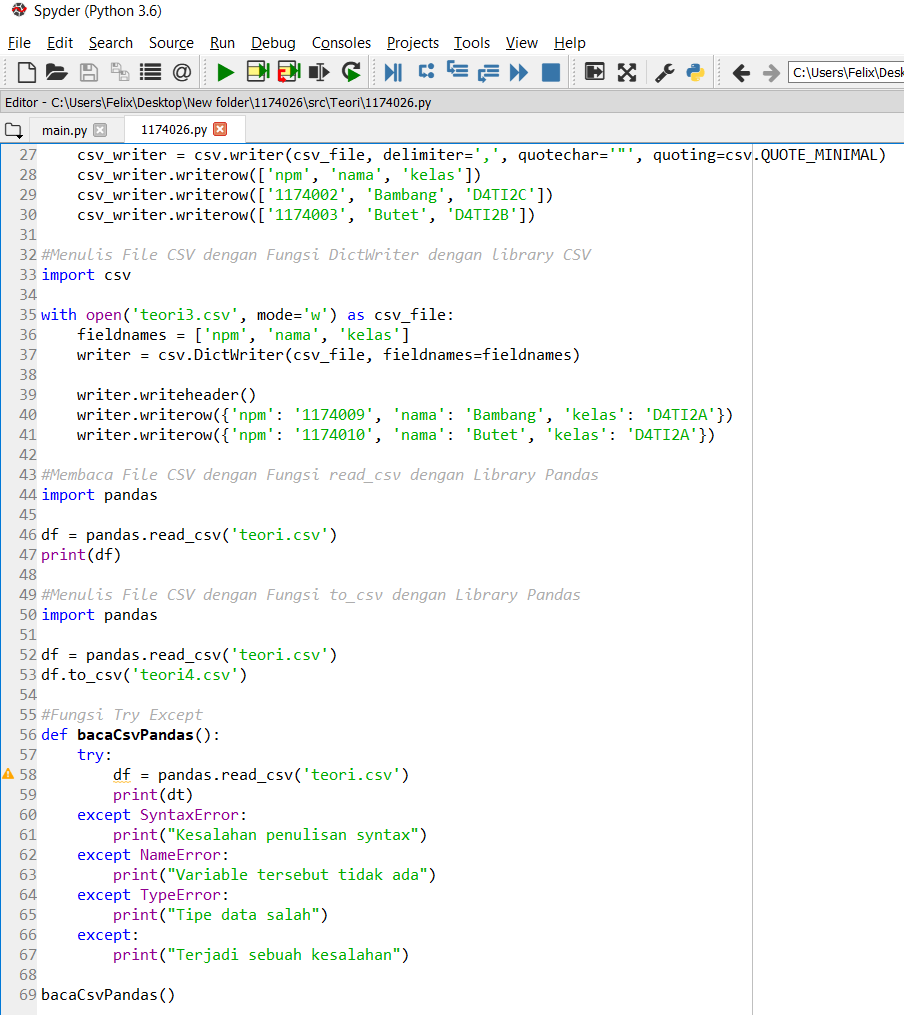
\includegraphics[width=10cm]{figures/4/1174026/Praktek/p1.png}
	\centering
\end{figure}

\subsection{Plagiat Penanganan Error}
\begin{figure}[H]
	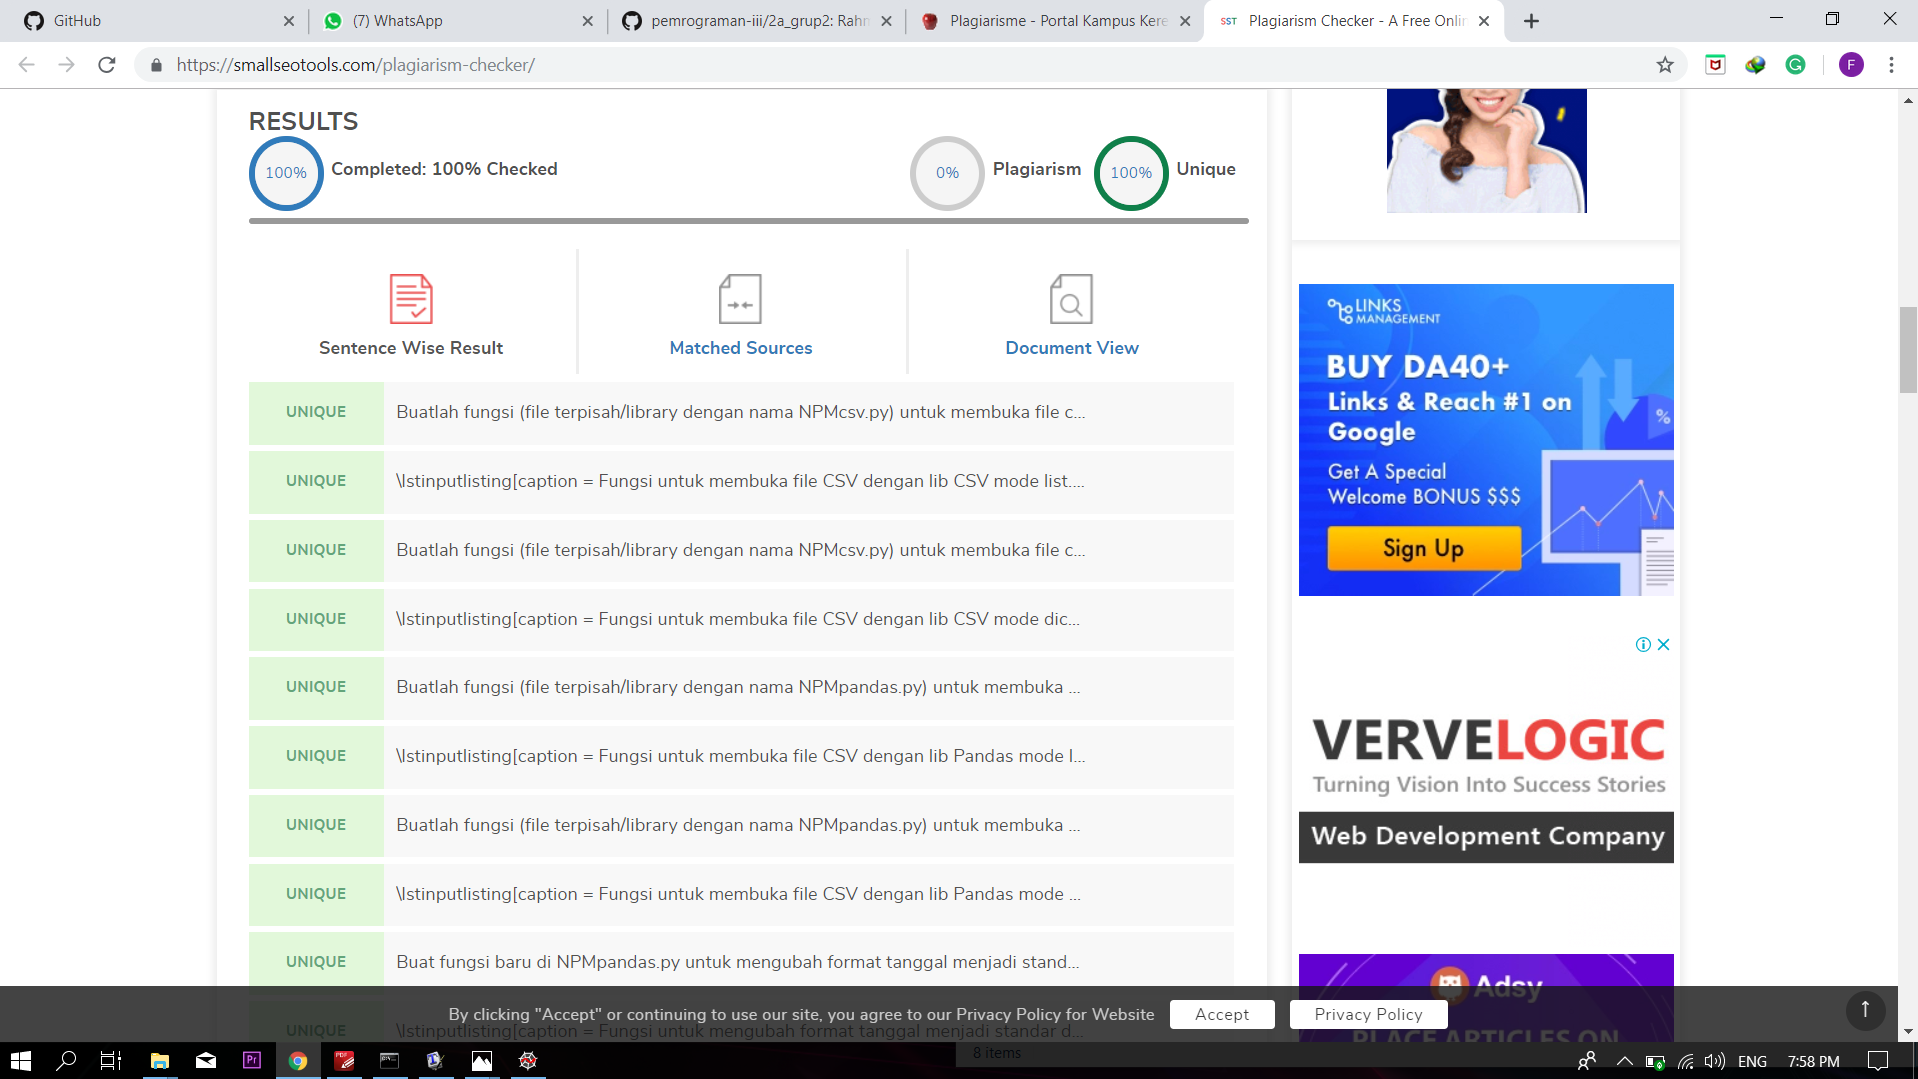
\includegraphics[width=10cm]{figures/4/1174026/Praktek/plagiatpenanganan.png}
	\centering
\end{figure}

%%%%%%%%%%%%%%%%%%%%%%%%%%%%%%%%%%%%%%%%%%%%%%%%%%%%

\section{Dwi Septiani Tsaniyah}
\subsection{Soal 1}
Buatlah  fungsi  (file  terpisah/library  dengan  nama  NPMcsv.py)  untuk  membuka file csv dengan lib csv mode list.
\lstinputlisting[firstline=9, lastline=21]{src/4/1174003/c_1174003_csv.py}

\subsection{Soal 2}
Buatlah  fungsi  (file  terpisah/library  dengan  nama  NPMcsv.py)  untuk  membuka file csv dengan lib csv mode dictionary.
\lstinputlisting[firstline=24, lastline=47]{src/4/1174003/c_1174003_csv.py}

\subsection{Soal 3}
Buatlah fungsi (file terpisah/library dengan nama NPMpandas.py) untuk membuka file csv dengan lib pandas mode list.
\lstinputlisting[firstline=10, lastline=11]{src/4/1174003/p_1174003_pandas.py}

\subsection{Soal 4}
Buatlah fungsi (file terpisah/library dengan nama NPMpandas.py) untuk membuka file csv dengan lib pandas mode dictionary.
\lstinputlisting[firstline=14, lastline=16]{src/4/1174003/p_1174003_pandas.py}

\subsection{Soal 5}
Buat fungsi baru di NPMpandas.py untuk mengubah format tanggal menjadi standar dataframe.
\lstinputlisting[firstline=19, lastline=20]{src/4/1174003/p_1174003_pandas.py}

\subsection{Soal 6}
Buat fungsi baru di NPMpandas.py untuk mengubah index kolom.
\lstinputlisting[firstline=23, lastline=24]{src/4/1174003/p_1174003_pandas.py}

\subsection{Soal 7}
Buat fungsi baru di NPMpandas.py untuk mengubah atribut atau nama kolom.
\lstinputlisting[firstline=27, lastline=42]{src/4/1174003/p_1174003_pandas.py}

\subsection{Soal 8}
Buat program main.py yang menggunakan library NPMcsv.py yang membuat dan membaca file csv.
\lstinputlisting[firstline=8, lastline=10]{src/4/1174003/main_dwi.py}

\subsection{Soal 9}
Buat program main2.py yang menggunakan library NPMpandas.py yang membuat dan membaca file csv.
\lstinputlisting[firstline=12, lastline=14]{src/4/1174003/main_dwi.py}

\subsection{Soal 1}
Tuliskan  peringatan  error  yang  didapat  dari  mengerjakan  praktek  keempat  ini, dan  jelaskan  cara  penanganan  error  tersebut.   dan  Buatlah  satu  fungsi  yang menggunakan gunakan try except untuk menanggulangi error tersebut.

Peringatan error di praktek keempat ini, yaitu:
\begin{itemize}
	\item Syntax Errors
	Syntax Errors adalah suatu keadaan saat kode python mengalami kesalahan penulisan. Solusinya adalah memperbaiki penulisan kode yang salah.
	
	\item Name Error
	NameError adalah exception yang terjadi saat kode melakukan eksekusi terhadap local name atau global name yang tidak terdefinisi. Solusinya adalah memastikan variabel atau function yang dipanggil ada atau tidak salah ketik.
	
	\item Type Error
	TypeError adalah exception yang akan terjadi apabila pada saat dilakukannya eksekusi terhadap suatu operasi atau fungsi dengan type object yang tidak sesuai. Solusi dari error ini adalah mengkoversi varibelnya sesuai dengan tipe data yang akan digunakan.
\end{itemize}



\section{Muhammad Fahmi}
\subsection{Soal 1}
	\lstinputlisting[caption=Soal 1., firstline=9, lastline=21]{src/4/1174021/Praktek/1174021_csv.py}
\subsection{Soal 2}
	\lstinputlisting[caption=Soal 2., firstline=24, lastline=55]{src/4/1174021/Praktek/1174021_csv.py}
\subsection{Soal 3}
	\lstinputlisting[caption=Soal 3., firstline=9, lastline=11]{src/4/1174021/Praktek/1174021_pandas.py}
\subsection{Soal 4}
	\lstinputlisting[caption=Soal 4., firstline=14, lastline=16]{src/4/1174021/Praktek/1174021_pandas.py}
\subsection{Soal 5}
	\lstinputlisting[caption=Soal 5., firstline=19, lastline=20]{src/4/1174021/Praktek/1174021_pandas.py}
\subsection{Soal 6}
	\lstinputlisting[caption=Soal 6., firstline=22, lastline=24]{src/4/1174021/Praktek/1174021_pandas.py}
\subsection{Soal 7}
	\lstinputlisting[caption=Soal 7., firstline=26, lastline=42]{src/4/1174021/Praktek/1174021_pandas.py}
\subsection{Soal 8}
	\lstinputlisting[caption=Soal 8.,firstline=8, lastline=10]{src/4/1174021/Praktek/main_fahmi.py}
\subsection{Soal 9}
	\lstinputlisting[caption=Soal 9., firstline=12, lastline=14]{src/4/1174021/Praktek/main_fahmi.py}
\subsection{Penanganan Error}
	\lstinputlisting[caption=Penanganan Error., firstline=8, lastline=11]{src/4/1174021/Praktek/errfahmi.py}
	
Peringatan error di praktek keempat ini, yaitu:
\begin{itemize}
	\item Syntax Errors
	Syntax Errors adalah suatu keadaan dimana saat kode python mengalami kesalahan penulisan. Solusinya adalah dengan memperbaiki penulisan kode yang salah.
	
	\item Name Error
	NameError adalah exception yang terjadi pada saat kode melakukan eksekusi terhadap suatu local name atau global name yang tidak terdefinisi. Solusinya adalah dengan memastikan variabel atau function yang dipanggil ada atau tidak salah ketik.
	
	\item Type Error
	TypeError adalah exception yang akan terjadi apabila pada saat melakukan eksekusi terhadap suatu operasi atau fungsi dengan type object yang tidak sesuai. Solusi dari error tersebut adalah dengan mengkoversi variabelnya sesuai dengan tipe data yang akan digunakan.
\end{itemize}

%%%%%%%%%%%%%%%%%%%%%%%%%%%%%%%%%%%%%%%%%%%%%%%%%%%%%%%%%%%%%%%%%%%

\section{Muhammad Tomy}
\subsection{Soal 1}
Buatlah  fungsi  (file  terpisah/library  dengan  nama  NPMcsv.py)  untuk  membuka file csv dengan lib csv mode list.

\lstinputlisting[caption = Fungsi untuk membuka file CSV dengan lib CSV mode list., firstline=10, lastline=15]{src/4/1174031/praktek/1174031csv.py}

\subsection{Soal 2}
Buatlah  fungsi  (file  terpisah/library  dengan  nama  NPMcsv.py)  untuk  membuka file csv dengan lib csv mode dictionary.

\lstinputlisting[caption =  Fungsi untuk membuka file CSV dengan lib CSV mode dictionary., firstline=17, lastline=22]{src/4/1174031/praktek/1174031csv.py}

\subsection{Soal 3}
Buatlah fungsi (file terpisah/library dengan nama NPMpandas.py) untuk membuka file csv dengan lib pandas mode list.

\lstinputlisting[caption =  Fungsi untuk membuka file CSV dengan lib Pandas mode list., firstline=10, lastline=13]{src/4/1174031/praktek/1174031pandas.py}

\subsection{Soal 4}
Buatlah fungsi (file terpisah/library dengan nama NPMpandas.py) untuk membuka file csv dengan lib pandas mode dictionary.

\lstinputlisting[caption =  Fungsi untuk membuka file CSV dengan lib Pandas mode dictionary., firstline=10, lastline=13]{src/4/1174031/praktek/1174031pandas.py}

\subsection{Soal 5}
Buat fungsi baru di NPMpandas.py untuk mengubah format tanggal menjadi standar dataframe.

\lstinputlisting[caption =  Fungsi untuk mengubah format tanggal menjadi standar dataframe., firstline=15, lastline=19]{src/4/1174031/praktek/1174031pandas.py}

\subsection{Soal 6}
Buat fungsi baru di NPMpandas.py untuk mengubah index kolom.

\lstinputlisting[caption =  Fungsi untuk mengubah index kolom., firstline=21, lastline=24]{src/4/1174031/praktek/1174031pandas.py}

\subsection{Soal 7}
Buat fungsi baru di NPMpandas.py untuk mengubah atribut atau nama kolom.

\lstinputlisting[caption =  Fungsi untuk mengubah atribut atau nama kolom., firstline=26, lastline=30]{src/4/1174031/praktek/1174031pandas.py}

\subsection{Soal 8}
Buat program main.py yang menggunakan library NPMcsv.py yang membuat dan membaca file csv.

\lstinputlisting[caption =  Membuat dan mebaca file CSV menggunakan library 1174031pandas., firstline=8, lastline=13]{src/4/1174031/praktek/main.py}

\subsection{Soal 9}
Buat program main2.py yang menggunakan library NPMpandas.py yang membuat dan membaca file csv.

\lstinputlisting[caption = Membuat dan mmebaca file CSV menggunakan library 1174031pandas., firstline=8, lastline=13]{src/4/1174031/praktek/main2.py}

\subsection{Soal 1}
Tuliskan  peringatan  error  yang  didapat  dari  mengerjakan  praktek  keempat  ini, dan  jelaskan  cara  penanganan  error  tersebut.   dan  Buatlah  satu  fungsi  yang menggunakan gunakan try except untuk menanggulangi error tersebut.

%%%%%%%%%%%%%%%%%%%%%%%%%%%%%%%%%%%%%%%%%%%%%%%%%%%%%%%%


\section{Harun Ar-Rasyid}
\subsection{Soal 1}
Isi jawaban soal ke-1

Kalau mau dibikin paragrap \textbf{cukup enter aja}, tidak usah pakai \verb|par| dsb

%\subsection{Soal 2}
%Isi jawaban soal ke-2

%\subsection{Soal 3}
%Isi jawaban soal ke-3

\section{Sri Rahayu}
\subsection{Soal 1}
Isi jawaban soal ke-1

Kalau mau dibikin paragrap \textbf{cukup enter aja}, tidak usah pakai \verb|par| dsb

%\subsection{Soal 2}
%Isi jawaban soal ke-2

%\subsection{Soal 3}
%Isi jawaban soal ke-3

\section{Doli Jonviter}
\subsection{Soal 1}
Isi jawaban soal ke-1

Kalau mau dibikin paragrap \textbf{cukup enter aja}, tidak usah pakai \verb|par| dsb

%\subsection{Soal 2}
%Isi jawaban soal ke-2

%\subsection{Soal 3}
%Isi jawaban soal ke-3

\section{Rahmatul Ridha}
\subsection{Soal 1}
Isi jawaban soal ke-1

Kalau mau dibikin paragrap \textbf{cukup enter aja}, tidak usah pakai \verb|par| dsb

%\subsection{Soal 2}
%Isi jawaban soal ke-2

%\subsection{Soal 3}
%Isi jawaban soal ke-3

\section{Tomy Prawoto}
\subsection{Soal 1}
Isi jawaban soal ke-1

Kalau mau dibikin paragrap \textbf{cukup enter aja}, tidak usah pakai \verb|par| dsb

%\subsection{Soal 2}
%Isi jawaban soal ke-2

%\subsection{Soal 3}
%Isi jawaban soal ke-3
